\documentclass[12pt]{article}
\usepackage{multicol}
\usepackage{sbc-template}
\usepackage{subfigure} 
\usepackage{float} 
\usepackage{graphicx,url}
\usepackage[brazil]{babel}   
%\usepackage[latin1]{inputenc}  
\usepackage[utf8]{inputenc}  
% UTF-8 encoding is recommended by ShareLaTex

     
\sloppy

\title{Oracle XML  Conceitos Básicos}

\author{Rafael Gonçalves de Oliveira Viana\inst{1} }


\address{Sistemas de Informação -- Universidade Federal do Mato Grosso do Sul
	(UFMS)\\
  	Caixa Postal 79400-000 -- Coxim-MS -- Brazil
  \email{rafael.viana@aluno.ufms.br}
}

\begin{document} 

\maketitle


     
\begin{resumo} 
  Este resumo demonstra como foi realizado o estudo e a construção do XML da aplicação Arsenal, proposta como atividade avaliativa da matéria de Danco de Dados II.
  
  
\end{resumo}


\section{Oracle Berkeley DB XML}

Como qualquer banco de dados normal, o Oracle Berkeley DB XML gera um banco de dados para XML em um arquivo em disco, com a extensão DBXML (Database XML) onde a sua aplicação através de uma API (Application Programming Interface) abre este arquivo, lê, escreve os dados e depois fecha. Como um arquivo convencional do sistema operacional.

Este simples conceito no Oracle Berkeley DB XML é chamado de Container, que funciona como uma área de memória  do banco de dados permitindo o gerenciamento dos arquivos XML de forma muito mais performática e ágil para à aplicação.\cite{dbxml}

Para acessar o BDB em sua máquina após a instalação, basta executar o comando DBXML ("Apenas consegui fazer funcionar no Windows"). Para criar um arquivo de container como na Figura \ref{fg1}, utliza-se o comando \textbf{CreateContainer}

	\begin{figure}[!htb]
	\centering
	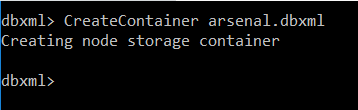
\includegraphics[scale=0.8]{./imagens/f1.png}
	
	\caption{Container arsenal}
	\label{fg1}
\end{figure}
\section{XML Schema}
XML Schema é uma linguagem de definição de esquema escrita em XML. Ele pode ser usado para descrever a estrutura e a semântica de documentos de instâncias. Um exemplo prático seria o modelo abaixo que representa um arsenal de armas.
	\begin{verbatim}
	<?xml version="1.0" encoding="utf-8" ?>
	<xsd:schema elementFormDefault="qualified"
	xmlns:xsd="http://www.w3.org/2001/XMLSchema">
	<xsd:element name="Arsenal" type="ArsenalType" />
	
	<xsd:complexType name="ArsenalType">
		<xsd:sequence minOccurs="0" maxOccurs="unbounded">
			<xsd:element name="Policial" type="ArmaType" />
			<xsd:element name="Arma" type="ArmaType" />
			<xsd:element name="valor_arma" type="xsd:number" />
			<xsd:element name="cadastro_criado" type="xsd:string" />
		</xsd:sequence>
	</xsd:complexType>
	
	<xsd:complexType name="ArmaType">
		<xsd:sequence>
			<xsd:element name="nome_arma" type="xsd:string" />
			<xsd:element name="categoria" type="categoria" />
			<xsd:element name="municao" type="municao" />
			<xsd:element name="fabricante" type="xsd:string" />
			<xsd:element name="modificacao" type="xsd:string" />
		</xsd:sequence>
	</xsd:complexType>
	
	<xsd:complexType name="categoria">
		<xsd:sequence>
			<xsd:element name="nome_categoria" type="xsd:string" />
			<xsd:element name="modificacao" type="xsd:string" />
		</xsd:sequence>
	</xsd:complexType>
	
	<xsd:complexType name="municao">
		<xsd:sequence>
			<xsd:element name="nome_municao" type="xsd:string" />
			<xsd:element name="calibre" type="xsd:string" />
			<xsd:element name="modificacao" type="xsd:string" />
		</xsd:sequence>
	</xsd:complexType>
	
	<xsd:complexType name="calibre">
		<xsd:sequence>
			<xsd:element name="nome_calibre" type="xsd:string" />
			<xsd:element name="restricao" type="xsd:string" />
			<xsd:element name="modificacao" type="xsd:string" />
		</xsd:sequence>
	</xsd:complexType>
	
	<xsd:complexType name="restricao">
		<xsd:sequence>
			<xsd:element name="nome_restricao" type="xsd:string" />
			<xsd:element name="nivel" type="xsd:string" />
			<xsd:element name="modificacao" type="xsd:string" />
		</xsd:sequence>
	</xsd:complexType>
	
	<xsd:complexType name="policial">
		<xsd:sequence>
			<xsd:element name="nome_policial" type="xsd:string" />            
			<xsd:element name="cod_policial" type="xsd:string" />
			<xsd:element name="matricula" type="xsd:string" />
			<xsd:element name="patente" type="xsd:string" />
			<xsd:element name="cadastro_criado" type="xsd:string" />
		</xsd:sequence>
	</xsd:complexType>
	</xsd:schema>
	\end{verbatim}
	
\section{Gerando XML atraves do Database}
	O exemplo abaixo descreve as funções padrão SQL / XML e as funções e pacotes fornecidos pelo Oracle Database para gerar dados XML a partir de conteúdo relacional. \cite{geracao}
	
	\begin{verbatim}
	select xmlelement("arsenal"
		,xmlattributes(arsenal.cod_arsenal as codigo)
		,xmlforest(arsenal.cod_arsenal as codigo)
		,xmlelement("policial"
			,(select xmlagg (xmlconcat(
				 xmlelement("nome",policial.nome_policial)
				,xmlelement("tel",policial.tel_policial)
				,xmlelement("matricula",policial.matricula)
				,xmlelement("cadastro_criado",policial.cadastro_criado)
				)
		)
			from policial 
			where arsenal.cod_policial = policial.cod_policial)
			)
		,xmlelement("arma"
			,(select xmlagg (xmlconcat(
				xmlelement("nome_arma",arma.nome_arma)
				,xmlelement("categoria",arma.categoria)
				,xmlelement("municao",arma.municao)
				,xmlelement("fabricante",arma.fabricante)
				,xmlelement("modificacao",arma.modificacao)
			)
		)
			from  arma, policial
			where policial.cod_arma = arma.cod_arma )
			)
		)
		,xmlelement("valor_arma",arsenal.valor_arma)
		,xmlelement("cadastro_criado",arsenal.cadastro_criado)     
		from  arsenal ;
	\end{verbatim}
Após o comando acima , o resultado foi o apresentado na Figura \ref{fg2}.
	\begin{figure}[H]
		\centering
		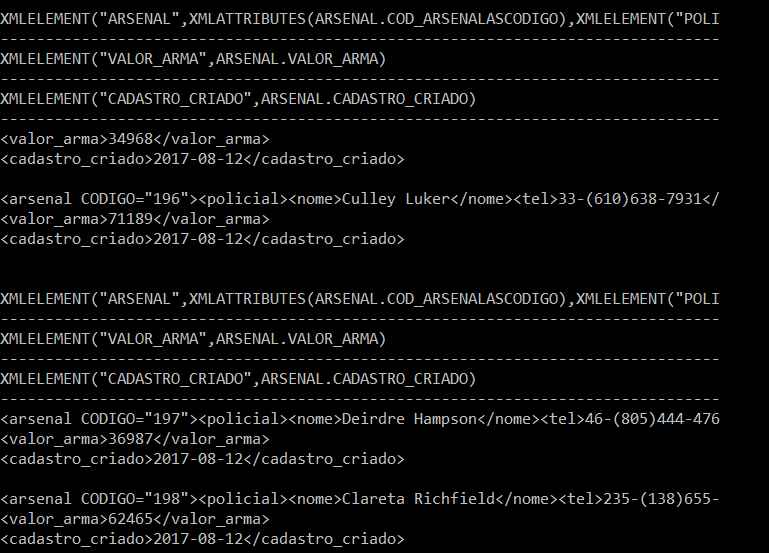
\includegraphics[scale=0.5]{./imagens/f2.png}
		\caption{Legenda}
		\label{fg2}
	\end{figure}
\section{Conclusão}
O XML é mesmo um grande aliado no desenvolvimento de aplicações avançadas para a Internet. O XML oferece um meio realmente eficiente de se transmitir dados de todo tipo através da rede.
	
\bibliographystyle{sbc}
\bibliography{sbc-template.bib}

\end{document}
